 \documentclass[10pt, conference, letterpaper]{IEEEtran}

\ifCLASSINFOpdf
	\usepackage[pdftex]{graphicx}
	\graphicspath{{./figures/}}
\else
  \usepackage[dvips]{graphicx}
  \graphicspath{{./figures/}}
\fi
	
\usepackage[cmex10]{amsmath}
\usepackage[caption = false, font = footnotesize]{subfig}
\usepackage{amsthm}
\usepackage{amsfonts}
\newtheorem{theorem}{Theorem}
\newcommand*{\rom}[1]{\uppercase\expandafter{\romannumeral #1\relax}} % new command to type upper case Roman numbers
%\usepackage[normlem]{ulem}
%\usepackage{algoithm}
%\usepackage{algpseudocode}
\usepackage{textcomp}
\usepackage{gensymb} % include degree mark


\DeclareMathOperator*{\argmax}{arg\,max}


\begin{document}
\title{Indoor mmWave Wearable Networks: Challenges to MAC Design}

\author{\IEEEauthorblockN{Yicong Wang and Gustavo de Veciana}
\IEEEauthorblockA{Department of Electrical and Computer Engineering, The University of Texas at Austin\\Email: yicong.wang@utexas.edu, gustavo@ece.utexas.edu }
}

\maketitle

\begin{abstract}
Millimeter wave (mmWave) serves as an ideal solution for wearable networks where device density can be high and many applications require Gbps throughput. In a dense scenario such as a crowded train or stadium, users are close to each other and the interference can be strong. Furthermore, wearable devices may have heterogeneous transmission capabilities and different Quality-of-Service (QoS) requirements. The wearable network in dense scenarios differs from other mmWave networks in two ways: (1) human body blockage and body movements make interferers have different interfering channels; (2) heterogeneity in device capabilities (e.g. beamforming v.s. omni-directional and different energy constraints) makes it inefficient to schedule all devices in the same way. Different scenarios poses challenges to the design of medium access control (MAC) protocols. In this paper, we begin with an analysis of the characteristics of interferers in dense wearable networks. We compute the number of strong interferers of a typical user and study the stability of strong interferers when users moves locally. We further show that when users make large scale movements, the channel state between two fixed points should be modeled as an $M/G/\infty$ queue instead of two-state Markov model. Based on our analysis of interferers, we discuss the hierarchical MAC to manage interference, including the clustering of users and scheduling at the user level. We propose clustering principles for wearables and analyze the performance of clustering and try to characterize the optimal cluster size of clusters for different scenmarios and device capabilities. We show that coexistence of heterogeneous devices present challenges and clustering and reuse can provide moderate gain in resource reuse but improves the probability of successful transmissions. 


\end{abstract}
\IEEEpeerreviewmaketitle

\section{Introduction}\label{section:introduction}
% Introduce problem
% 1. Introduce potential challenges of channel: high density of users, mmWave channel
% 2. Existing work on modeling and analysis of interference
% Lacks channel characterizaion for MAC design in "dense" "wearable" network
% 3. MAC design challenges and existing solutions
% Contributions:
% 1. Analysis of channels
% 2. Hierarchical MAC
% 3. Analysis of MAC and propose suggestions on MAC

% 1. Brief introduction
The market for wearable devices is growing fast in recent years \cite{wearable} and research on wearable networks is now being actively pursued.  Users are equipped with multiple wearable devices on the body with the devices of a user communicating with each other. To support the high data rates and high density of wearable devices, millimeter wave communication serves as a good solution and standards have been developed for short-range wireless personal area network (WPAN) in mmWave, e.g., 802.11ad \cite{80211ad}, 802.15.3c \cite{802153c} and ECMA387 \cite{ECMA387}. 

In dense wearable network with high user density, e.g., a train car or a crowded stadium, the number of interferers is high and the existing protocols may fail to coordinate the vast number of WPANs and meet the QoS requirements of different devices efficiently due to high density of interferers and highly variable channels. The design of medium access control (MAC) for dense and heterogeneous wearable networks requires understanding of characteristics of interference environment and the requirements of different devices.

% 2. Modeling and analysis of interference
Two major factors influencing the interference environment in dense wearable networks are human blockage and user movements. Human body introduces a path loss of over 20dB \cite{humanshadowing} thus the variation in channel gain is large. \cite{urbanblockage} analyzes blockage effect in urban area and compute the penetration loss of the path using stochastic geometry tools. \cite{interferencefinitesized} studies the human shadowing effects in finite-sized area where the locations of users are fixed. The authors uses different path loss exponents and fading models to model the LOS and NLOS channels and compute the SINR distribution. \cite{enclosedmmwave} model the wearable network in enclosed environment and the reflected channels are considered to compute the signal-to-interference-ratio (SINR) distribution of channels. The analysis of the interference in mmWave mainly focus on the distribution of SINR and assume the users are uncoordinated. Users either transmit all the time or use simple MAC protocols, e.g., Aloha. 

Another important feature of dense wearable network is that channels are more sensitive to user movements, including small local movement like turning torso or swinging and large scale movement, e.g., people walking around. Existing work on the user mobility of users \cite{humanactivity}\cite{blockagein60ghz}\cite{timevaryingpathshadowing} study the influence of human mobility on the radio channel between fixed transmitter and receiver. \cite{humanactivity}\cite{timevaryingpathshadowing} present measurements on the impact of human mobility and show that human movements causes variations in channel. \cite{timevaryingpathshadowing} further compute the probability that channel is blocked by users and model the state of channel using two states Markov model. 
%(More work using Markov model, reference required)
\cite{blockagein60ghz} use simulations to get the radio propagation in the presence of static and moving obstacles and show that directional LOS wave links experience relatively high outage. These works provide valuable measurements and insights on the influence of moving human blockage, but they do not provide tractable analysis of user movements to quantify the influence of user mobility.

%In wearable network, the TXs and RXs are on the user's body thus the model channels between users are either interfering channels or used for signaling.   while user movements mainly affect the interference to a user instead of signal channel. Furthermore, the high density of users and different mobility patterns in wearable network affect the interference environment.

% 3. New challenges to MAC design
% 1) Large number of users to deal with (signaling) Existing standards, protocols aiming at improving reuse
% 2) (Combine 2 to 1)Interference is higher, wired model does not hold
% 3) *Blockage is different
% 4) Mobility: large scale, small scale
% 5) Heterogeneity of devices

% Contributions: describe our work


% What are important in the analysis of interference. Move this to contributions
From the MAC design perspective, it is important to identify the set of interferers users need to deal with, i.e., the set of strong interferers. We define \emph{strong interferer} of a user as a neighboring user whose device has a strong channel to the user. The channel of a strong interferer can be an LOS channel, or a strong reflected channel. Understanding the set of strong interferers will help us identify the users that MAC need to keep track of and coordinate.

We first provide an analysis of the set of strong interferers. We model the users as a marked point process (m.p.p.) and identify the set of strong interferers of a typical user. We further model the interferers using a homogeneous Poisson Point Process (P.P.P.) and compute the expected number of strong interferers. We show that the number of strong interferers is actually limited as user density increases and a typical user sees most strong interferers at moderate high density. We give the spatial distribution of strong interferers and show that strong interferers will concentrate to the typical user for high user density scenario. We then consider the influence of different scales of user movements, i.e., small local movements and large scale constant velocity movements. For small local movements, we use the sensitivity of strong interferers and show that distant users are more unstable than close interferers. We also show that the set of strong interferers are most sensitive when user density is moderate high, assuming that the range of local movements is limited for high user density. For large scale movements, we model that users moves at constant velocities and study the state transition of a fixed channel. We prove that the state of the channel follows a $M/G/\infty$ queue instead of the simple Markove model with two states and the distribution of intervals of being blocked has a heavy tailed distribution(?). We further compute the average length of intervals of having a strong channel  and the intervals that the channel is blocked.


We then discuss the hierarchical MAC in wearable networks. Clustering and channel selection can be used to mitigate interference while scheduling at each user can be used to schedule wearable devices and improve channel reuse by learning the transmission patterns of other users.

Thirdly, we discuss the principles and design objectives of clustering. To evaluate clustering, we model clustering and FDM scheme and analyze the network capacity based on our analysis of strong interferers. We show how the optimal cluster size and the capacity of the network changes for different scenarios, e.g., user density, transmission capabilities and traffic patterns of users.


%Strong interferer is defined as Close neighbors of a user may block the channel between a user and his distant neighbors, decreasing the number of potential interferers. Self-blockage also contributes to reducing interference from neighbors. However, the locations of users are not fixed over time and even small movements like turning the torso or stretching the limb can dramatically change the interference environment a user see.  Generally, the channel between two close neighbors are less likely to be interfered by the local movements of users while a long channel are more sensitive to motion. 

%In this paper, we address the problem of MAC design for dense indoor mmWave wearable networks with heterogeneous devices. The wearable devices on a user's body form a wireless personal area network (WPAN), with a device working as the coordinator of the WPAN and all other devices communicating with the coordinator. A good candidate of coordinator is the smart phone which has access to the Internet and is equipped with smart antennas. In 802.11ad, such directional multi-gigabit (DMG) basic service set is defined as personal basic service set (PBSS) and the coordinator station is called personal basic service set control point (PCP)/access point(AP). We will use the same terminology for wearable network as 802.11ad in our paper. 

%The transmission capabilities and QoS requirements of wearable devices can be heterogeneous in wearable networks. There are high-end devices equipped with smart antennas having high QoS requirements, e.g., smart glasses supporting augmented reality. High-end devices will be interfering with fewer devices since their transmission is directional but may fail to meet the QoS requirements once interfered. On the other hand, there are low-end devices that do not support highly directional beamforming and transmit in quasi-omni directional mode, e.g., smart jewelries and pedometers. Low-end devices transmit at lower rates and have no strict requirements on delay but can not try to transmit all the time due to energy limit. 


%The heterogeneous requirements of devices and unique characteristics of highly dense wearable networks inspire us to rethink the MAC design principles. The high density of devices require spatial reuse of resources but the omni-directional transmissions, e.g., beacon transmission and low-end transmissions, and the fast changing interference channels make it hard to achieve spatial reuse with existing techniques like beam alignment. The heterogeneity in wearable devices indicates that different types of transmissions can and perhaps should be treated differently in MAC scheduling. In this paper, we want to design an efficient distributed MAC protocol to meet the requirements of heterogeneous wearable devices in highly dense wearable networks based on mmWave links.

%\emph{Contributions}
%We present an analysis of the interference environment in highly dense wearable network and devise distributed MAC protocols to coordinate the PBSSs which provide higher resource utilization gain than TDMA and meet the QoS requirements of heterogeneous devices. The key idea of our scheduling method is to reserve resource for the transmission of high-end devices while low-end devices try to learn the channel and reuse the resource. 


\section{Interference in Dense Wearable Network}\label{section:channel}
In highly dense wearable networks, a user has a large number of neighbors in close proximity, but there are several factors limiting the actual number of interferers a user sees at one time, including the shadowing of human body, directional transmissions and upward-downward directionality of wearable network. The factors Also, directional transmissions will limit the width of beam and a user will be interfering with fewer other users. The upward-downward directionality comes from the general posture of humans and location of common wearable devices. Many devices are located along the torso instead of around the torso thus when directional transmission is used, transmission is in upward or downward direction, reducing the probability of interfering with other users. 

The exact modeling of the channels, especially the NLOS channels is still an open question and there has been quite a few works on channel modeling for mmWave, using channel modeling and/or measurements. In our analysis, we assume human body blockage will block the interference channel and we further consider one time reflection over the ceiling.We ignore the intractable reflection or scattered interference channels in our analysis.
 
\subsection{Number of Strong Interferers}
We try to analyze the set of strong interferers seen by a typical user. The typical user is located at the origin of a 2-D plane, with all the other users standing on the plane. There is no walls or obstructions other than human body, and there is a ceiling at $H$. The human body is modeled as cubics as shown in Fig. {figure of body model} and the locations of the users follow a point process $\Phi=\{x_i\}_i$, where $x_i$ is the location of user $i$. The PCP device is located in front of the human body, at the height of 1m and the facing direction of user $i$ is $\theta_i$. 

The interferers are determined by the location and orientation of the users and the other users can be modeled using a marked point process (m.p.p.) $\tilde{\Phi}=\{(x_i, \theta_i)\}_i$. For a typical user located at the origin facing direction $\theta_0$, the number of strong interferers given $\tilde{\Phi}$ is as follows,
\begin{equation}
N_{\mathrm{SI}}(\tilde{\Phi}, \theta_0) = \sum_{(x_i, \theta_i)\in \tilde{\Phi}}f_0(x_i, \theta_i, \tilde{\Phi}\backslash\{(x_i,\theta_i)\}, \theta_0)
\end{equation}
where $f_0(x_i, \theta_i, \tilde{\Phi}\backslash\{(x_i,\theta_i)\}, \theta_0)$ is the indicator function that whether $u_i$ is a strong interferer of the typical user located at the origin, considering the locations and orientations of $u_i$, $(x_i, \theta_i)$, the orientation of the typical user, $\theta_0$, and blockages from other users, $\tilde{\Phi}\backslash\{(x_i,\theta_i)\}$. 

For LOS interferers, $f_0$ is $1$ if the distance between devices is close enough and the interfering channel is not blocked by the typical user, the interferer and other interferers. For NLOS strong interferers, e.g., interferer with a strong reflection over the ceiling, we need to consider human body blockage, channel path loss as well as the reflection. 

$N_{\mathrm{SI}}$ varies for different scenarios and the its distribution is hard to compute. The average number of strong interferers works as a good metric to understand the requirements on MAC. If we assume that the orientations of users are mutually independent, then the interferers form an independent marked point process. Using the Campbell-Mecke theorem, the expected number of strong interferers $\mathrm{E}[N_{\mathrm{SI}}]$ can be expressed as, 
\begin{equation} \label{eq:N_SI}
\begin{split}
\mathrm{E}[N_{SI}] &= \mathrm{E}^0\bigg[\int\limits_{\mathbb{R}^2\times\mathbb{R}}f_0(x_i, \theta_i, \tilde{\Phi}\backslash\{(x_i,\theta_i)\}, \theta_0)\tilde{\Phi}(\mathrm{d}(x,\theta)) \bigg]\\
&= \int\limits_{\mathbb{R}^2}\int\limits_{\mathbb{R}}\int\limits_{\mathbb{\tilde{M}}}\mathrm{E}_{\theta_0}[f_0(x,\theta,\tilde{\phi}, \theta_0)]P_{(x,\theta)}^{!}(\mathbb{d}\tilde{\phi})F_x(\mathbb{d}\theta)M(\mathbb{d}x)
\end{split}
\end{equation}
where $\mathrm{E}^0$ is the expectation given that there is a user at the origin, $\mathrm{E}_{\theta_0}$ is taking the expectation over $\theta_0$, $P_{(x,\theta)}^!$ is the palm distribution of marked point process given that there is a point $(x, \theta)$ and a point at the origin. $F_x(\theta)$ is the CDF function of orientation for a user located at $x$ and $M(x)$ is the CDF function that a user is located at $x$. 

For tractability, we use homogeneous Poisson Point Process to approximate the locations of users. The facing directions of users are independent of user locations and uniformly distributed in $[0, 2\pi)$. Given these assumptions, the number of users that may block the interference channel follows Poisson distribution and the expected number of strong interferers, $\mathrm{E}[N_{\text{SI}}]$, is shown as follows, 
\begin{equation}
\begin{split}
\mathrm{E}[N_{\text{SI}}] & = P_{\text{facing}}\int\limits_{\mathbb{R}^2\backslash\mathrm{B}(0,r_{\text{min}})}
\text{1}(|x|<R_{\text{max}})e^{-\mathrm{E}[N_{\mathrm{B}}(x)]}\lambda(\mathrm{d}x)\\
&= 2\pi\lambda P_{\text{facing}}\int\limits_{\mathrm{r_{min}}}^{\mathrm{r_{max}}}e^{-\lambda\cdot\mathrm{E}[D]\cdot r}r\mathrm{d}r
\end{split}
\end{equation}
where $P_{\text{facing}}$ is the probability of the two users are not blocked by the bodies of the two users, $r_{\mathrm{min}}$ is the minimum distance between the centers of the users. $N_{\mathrm{B}}(x)$ is the number of users that blocks the interference channel from user located at $x$.
\begin{equation} \label{eq:N_blockage_original}
\begin{split}
\mathrm{E}[N_{\mathrm{B}}(x)] &= \int\limits_{\mathbb{R}^2}\int\limits_{[0,2\pi)}\mathrm{1}((x',\theta')\mathrm{~blocks~}(x,\theta))F_{\theta'}(\mathrm{d}\theta')\lambda(\mathrm{d}x') \\
& = \lambda|x|\int\limits_{\mathbb{R}}\int\limits_{[0,2\pi)}\mathrm{1}(d(\theta')<2h)\mathrm{d}\theta'\mathrm{d}h \\
& = \lambda|x|\mathrm{E}[D]
\end{split}
\end{equation}
where $h$ is the distance between the center of blockage to the line between the origin and $x$, $\mathrm{E}[D]$ is the expected width of a user that may block the channel between the origin and user $x$.

$\mathrm{E}[N_{\mathrm{SI}}]$ for different user densities is plotted in Fig. \ref{fig:Channel_en_si}. The average number of LOS and NLOS interferers are given and the results is compared to results from simulations where the locations of users follow Mat\'ern \rom{3} process \cite{matern} instead of Poisson Point Process. Analytical results are in line with the simulations, validating the accuracy of the analytical model. 

\begin{figure}
	\centering
	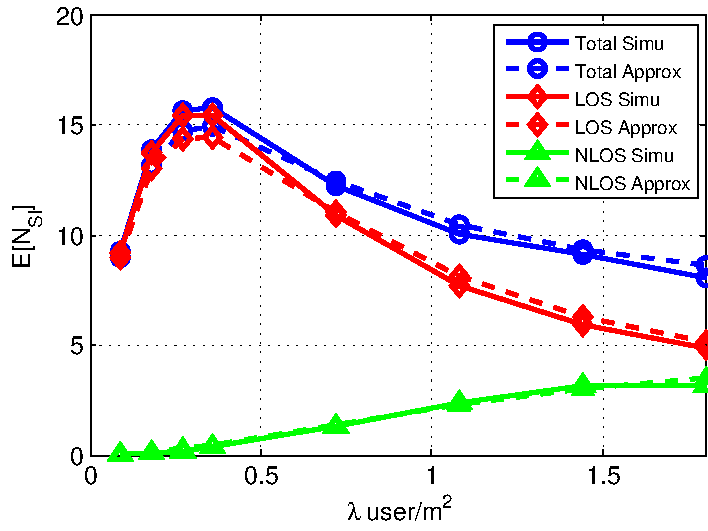
\includegraphics[width = 0.4\textwidth]{Channel_en_si.pdf}
	\caption{$\mathrm{E}[N_{\mathrm{SI}}]$ for different user densities.}
	\label{fig:Channel_en_si}
\end{figure}


\begin{figure}
	\centering
	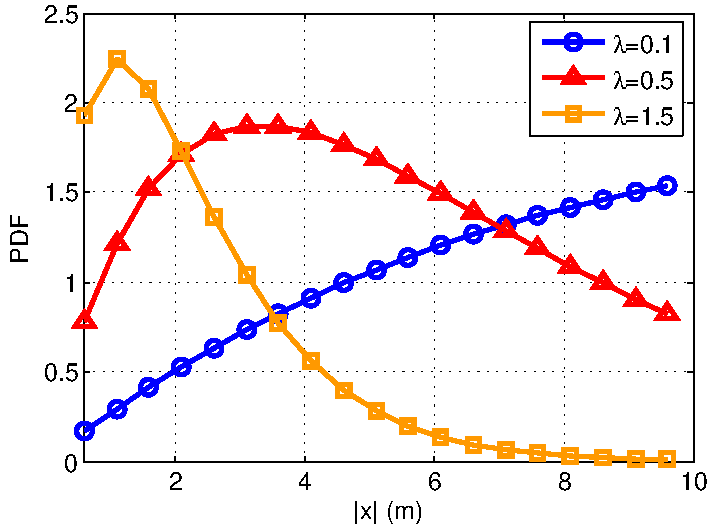
\includegraphics[width = 0.4\textwidth]{Channel_si_pdf.pdf}
	\caption{Probability density function of LOS strong interferers as a function of distance to $\bf{0}$.}
	\label{fig:Channel_si_pdf}
\end{figure}

$\mathrm{E}[N_{\mathrm{SI}}]$ first grows as the user density increases. As user density further increases, users closely around the typical user forms a wall blocking the interference channels from distant interferers. Users see most strong interferers at moderate high user density, instead of high user density scenarios. Fig.  illustrates how the set of strong interferers are as the user density increases, self blockage is not considered. In high density scenario, the number of users the MAC need to coordinate at the same time is actually limited, indicating that it is possible to mitigate interference in highly dense scenario using MAC to coordinate the users.

\subsection{Sensitivity of Strong Interferers}
Interference channels are sensitive to user movements, especially for dense wearable networks. The sensitivity of strong interferers defines the cost and benefit of keep tracking of and coordinating the strong interferers and how robust the strong interferers are to perturbations in the network. From $t$ to $t+\Delta t$, the users make translations as well as rotations, the changes for the typical user and potential interferers are shown as follows:
\begin{equation*}
\begin{split}
(0,\theta_0)&\rightarrow(\Delta x_0, \theta_0 + \Delta\theta_0) \\
\tilde{\Phi}_{t}=\{(x_i, \theta_i)\}&\rightarrow\tilde{\Phi}_{t+\Delta t}=\{(x_i+\Delta x_i, \theta_i + \Delta\theta_i)\}
\end{split}
\end{equation*}

Let $Y_x^t=f_0(x, \theta, \tilde{\Phi}_t\backslash (x, \theta), \theta_0)$ be the state of an interferer located at $x$ at time $t$, and $Y_x^{t+\Delta t}$ the state of the user at $t+\Delta t$ is given by,
\begin{multline*}
Y_{x}^{t+\Delta t} = f_{\Delta x_0}(x+\Delta x, \theta + \Delta\theta, \tilde{\Phi}_{t+\Delta t}\backslash (x+\Delta x, \theta + \Delta\theta), \\
\theta_0 + \Delta\theta_0).
\end{multline*}

We define the sensitivity of an interferer originally located at $x$, $S(x)$, as the autocorrelation of states of an interferer at $t$ and $t+\Delta t$. 
\begin{equation}
S(x, \Delta t)
=\mathrm{Corr}(Y_x^t, Y_x^{t+\Delta t})
=\frac{\mathrm{E}[Y_x^t\cdot Y_x^{t + \Delta t}]}{\sigma_{Y_x^t}\cdot \sigma_{Y_x^{t+\Delta t}}}
\end{equation} 

Notice that the state transition is not a Markovian process. We will explain this in detail in section \ref{subsection:largemobility}.

Assuming the network is stable and users movements are independent from each other, the variance of $Y_x^t$ and $Y_x^{t+\Delta t}$ are given by,
\begin{equation*}
\mathrm{Var}(Y_x^t)=p_{\mathrm{SI}(x)}\cdot (1-p_{\mathrm{SI}}(x)),
\end{equation*}
where $p_{\mathrm{SI}}=\mathrm{Pr}(f_0(x,\theta,\tilde{\Phi}\backslash\{(x_i,\theta_i)\}, \theta_0)=1)$. 
The sensitivity of users can be computed by computing the probability that the user remains a strong interferer after perturbation, $\mathrm{Pr}(\{Y_x^t=1\}\cap \{Y_x^{t+\Delta t}=1\})$. Define a user $(x',\theta')$ be a possible blockage if this user blocks the interference channel between the origin and $(x,\theta)$ at $t$ at $t$ or blocks the channel after perturbation at $t+\Delta t$. For given $(\Delta x_0, \Delta\theta_0)$ and $(\Delta x, \Delta\theta)$, the distribution of possible interferers follows a Poisson Point Process, thus the probability of being a strong interferer is given by
\begin{multline}
\mathrm{Pr}(\{Y_x^t=1\}\cap \{Y_x^{t+\Delta t}=1\}|(\Delta x_0, \Delta \theta_0), (\Delta x, \Delta\theta))=\\
e^{-\mathrm{E}[N_{\mathrm{PB}}(x)|(\Delta x_0, \Delta \theta_0), (\Delta x, \Delta\theta)]}\cdot
\mathrm{P}_{\mathrm{facing}}^{\ast}(\Delta \theta_0, \Delta\theta)
\end{multline}
where $N_{\mathrm{PB}}(x)$ is the number of possible blockages, $\mathrm{P}_{\mathrm{facing}}^{\ast}(\Delta \theta_0, \Delta\theta)$ is the probability that the interferer and the typical user are facing each other before and after perturbation. 

To model the movements of users, we assume the translation of a user is uniformly distributed in a circle around the user, $\Delta x \sim \mathrm{unif}(\mathcal{B}(0, r(\Delta t)))$. $r(\Delta t)$ is the maximum range of perturbation and is related to $\Delta t$. Users also rotate by some random angle $\Delta \theta \sim \mathrm{unif}[-\omega(\Delta t), \omega(\Delta t)]$, where $\omega(\Delta t)\in[0,\pi]$ is the maximum range of rotation. When user density is moderate high, we assume the perturbation range remains the same. As user density increases, the distance between users becomes smaller and the range of translation actually becomes smaller as user density increases. The range of translation is shown in Fig. \ref{fig:Channel_translation_range}, while the range of rotation remains the same, $\omega=24\degree$, which is $1/10$ of the angle not blocked by self-blockage.

\begin{figure}
	\centering
	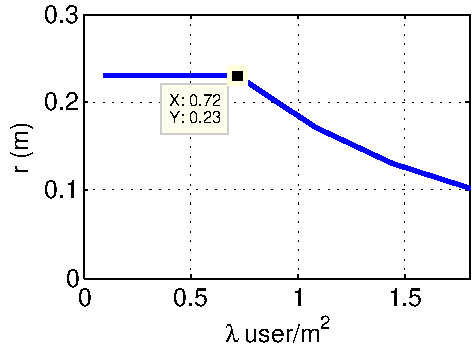
\includegraphics[width = 0.3\textwidth]{Channel_translation_range.pdf}
	\caption{Range of translation $r$ for different user densities $\lambda$}
	\label{fig:Channel_translation_range}
\end{figure}

In Fig. \ref{fig:Channel_sensitivity}, we show the sensitivity of users at different locations. Distant interferers are more sensitive to perturbations than close interferers, showing that close interferers learning the interference from close neighbors is more reliable. The sensitivity decreases as user density increases when density is low, i.e., below 0.72. As user density further increases, the sensitivity relatively stays the same as the range of movement decreases. In Fig. \ref{fig:Channel_sensitivity_average} shows how the average sensitivity of strong interferers changes for different user densities. When user density increases, strong interferers are closer while the sensitivity of users decreases, thus the average sensitivity first decrease with user density. When the range of limitation starts to decrease, the sensitivity of users remains the same while $\mathrm{E}[S]$ increases as strong interferers are closer. The above results shows that interferers are more sensitive to perturbation, and thus harder to keep track of as user density increases and the worst case happens at moderate high user density scenario, where the number of strong interferers is high and the range of perturbation is not limited by high user density. 

\begin{figure}
	\centering
	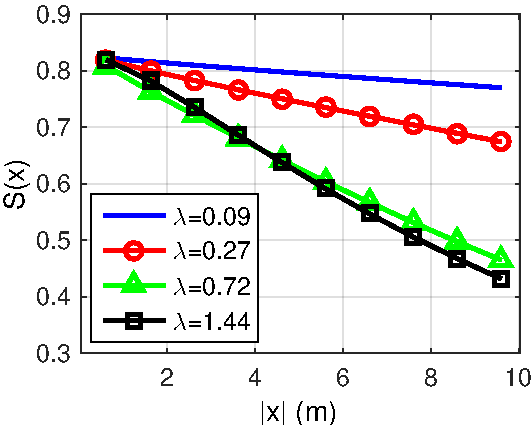
\includegraphics[width = 0.4\textwidth]{Channel_sensitivity.pdf}
	\caption{Sensitivity of users at different locations.}
	\label{fig:Channel_sensitivity}
\end{figure}
\begin{figure}
	\centering
	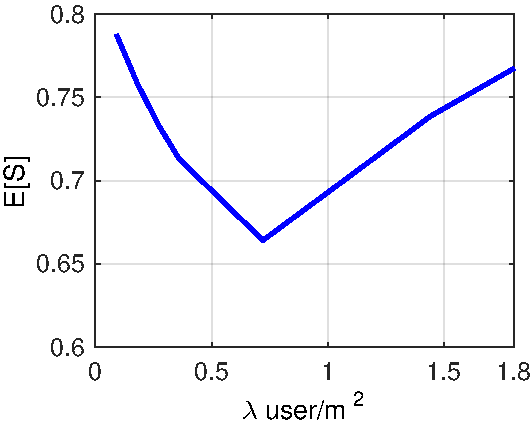
\includegraphics[width = 0.3\textwidth]{Channel_sensitivity_average.pdf}
	\caption{$\mathrm{E}[S(x)|f_0(x_i, \theta_i, \tilde{\Phi}\backslash\{(x_i,\theta_i)\}, \theta_0)=1]$ average sensitivity of strong interferers.}
	\label{fig:Channel_sensitivity_average}
\end{figure}


\subsection{Influence of Large Scale Mobility}\label{subsection:largemobility}
Another scenario we are interested in is dense user environment where users moves, e.g., populated streets. For large scale mobility, we focus on the influence of human blockage and show the transition of channel states between LOS and blocked. Let ${OX}$ be the channel between the target user and his neighbor $x$. ${OX}$ is fixed while other users move towards random directions at constant speeds. We assume the initial distribution of users follows a homogeneous Poisson Point Process with density $\lambda$, the directions of users are uniformly distributed over $[0,2pi)$ and the speed of each user $x$, $v$, is fixed. Then each user is uniquely decided by $(x, v, \theta)$. At any time $t$, the locations of users still follow a homogeneous Poisson Point Process with density $\lambda$.

For any time interval $[t, t + \Delta t]$, each user $x$ will cover a rectangular area $A_x$ as shown in Fig. \ref{fig:boolean}. ${OX}$ will remain LOS if there is no user intersects with ${OX}$ during the interval. The locations of users at $t$ follows a Poisson distribution, the areas covered during $\Delta t$ are independent and identically idistributed (i.i.d.), thus the coverage areas of users forms a Boolean model. For Boolean model, the number of sets that intersects with a fixed convex set follows Poisson distribution, thus the number of users blocking ${OX}$ during $[t, t+\Delta t]$ follows a Poisson distribution with mean
\begin{equation}
\mathrm{E}[N_{blockage}^{\Delta t}]=\lambda\big(\mathrm{E}[\nu(A_0^{\Delta t})] + \frac{1}{\pi}\nu_1({OX})\mathrm{E}[\nu_1(\partial A_0^{\Delta t})]\big)
\end{equation}
where $A_0^{\Delta t}$ is the typical coverage area for $\Delta t$, $\nu$ is the two-dimensional measure of the area, $\nu_1$ is the one-dimensional measure, $\partial A_0$ is the boundary of $A_0$. Assuming the speed and direction of each user is constant and the shape of users are convex, then 
\begin{equation*}
\begin{split}
\mathrm{E}[\nu(A_0^{\Delta t})] & = w\cdot (d + \mathrm{E}[v]\Delta t) \\
\mathrm{E}[\nu_1(\partial A_0^{\Delta t})] & = 2(w+d+\mathrm{E}[v] \Delta t)
\end{split}
\end{equation*}

The number of blockage during the interval follows an Poisson distribution, the users are independent from each other and the time that a user blocks $OX$ is independent from all other users. As a result, we can model the number of users blocking $OX$ as an $M/G/\infty$ queue. (Add a theorem or provide some proof?)
The arrival rate of blockage is given by $\lambda\mathrm{E}[v](w+\frac{2|OX|}{\pi})$. The distribution of time that a user blocks $OX$ is decided by the distribution of speed $v$.

Let $T_{\mathrm{LOS}}$ be the length of an interval that $\mathbf{OX}$ is an LOS channel and $T_{\mathrm{NLOS}}$ be the length of the interval that $OX$ is blocked by at least one users. From the analysis of the $M/G/\infty$ queue, $T_{\mathrm{LOS}}$ follows a exponential distribution with parameter $\lambda\mathrm{E}[v](w + \frac{2|OX|}{\pi})$, then
\begin{equation}
\mathrm{E}[T_{LOS}]  = \frac{1}{\lambda\mathrm{E}[v](w + \frac{2|OX|}{\pi})}
\end{equation}


We can then compute the probability that $OX$ is clear at any time $t$, 
\begin{equation}
\mathrm{P}_{\mathrm{LOS}} = e^{-\mathrm{E}[N_{blockage}^0]}
\end{equation}
where 
\begin{equation*}
\mathrm{E}[N_{blockage}^0] = \lambda\big(wd+\frac{2|OX|}{\pi}(w+d)\big)
\end{equation*} 
is the expected number of users overlapping with $OX$. Notice that here we do not consider the fact that the typical user and receiver will not overlap with blockages, thus $\mathrm{E}[N_{blockage}^0]$ is a different approximation from the result in (\ref{eq:N_blockage_original}).

From queuing theory, 
\begin{equation}
\frac{\mathrm{E}[T_{\mathrm{LOS}}]}{\mathrm{E}[T_{\mathrm{LOS}}] + \mathrm{E}[T_{\mathrm{NLOS}}]} = \mathrm{P}_{\mathrm{LOS}}
\end{equation}
\begin{equation}
\mathrm{E}[T_{\mathrm{NLOS}}] = \frac{1-\mathrm{P}_{\mathrm{LOS}}}{ \mathrm{P}_{\mathrm{LOS}}}\mathrm{E}[T_{\mathrm{LOS}}]
\end{equation}

Our analysis show that the state of $OX$ is not a simple Markov process with only two states but a $M/G/\infty$ queue. The distribution of the time that $OX$ is blocked shows heavy tailed distribution, indicating that $\mathrm{E}[T_{\mathrm{NLOS}}]$ can be very long. In some cases, the channel between two links can be blocked for a long time. For general indoor communications, this shows that outage due to blockage of 60 GHz communication can be worse than the result in analytical model. For dense wearable networks, long $T_{\mathrm{NLOS}}$ will result in reorganization of the users, thus the frequency of changing topology can be higher than that in Markov model.





\newpage
newpage
\newpage

\section{Clustering and Channel Selection}
Clustering improves spatial reuse and reduce interference \cite{80211ad}. Cluster head synchronizes the cluster members and schedules beacon transmissions in the cluster to mitigate intra-cluster interference, while other techniques like channel selection (FDM) and back off \cite{backoff} can be used to reduce inter-cluster interference. The 802.11ad Standard provides both distributed clustering and centralized clustering methods for directional devices working on mmWave. The links between PCPs/APs are unstable in dense wearable networks, thus the distributed clustering method fits better and we will use the distributed clustering algorithm in 802.11ad as the baseline.

In the distributed clustering algorithm, the formation of cluster follows a first come first serve rule: a BSS tries to join a existing cluster when it enters a network and starts a new cluster if no existing cluster is available. The maintenance of clusters is similar to lowest ID clustering. If the original cluster head is lost or two clusters meet each other, the remaining BSS or the original cluster head with the lowest/lower ID will be selected as the new cluster head. The Beacon SPs of cluster members are non-overlapping in time and a BSS need to reserve the slots if the PCP/AP or other devices receive beacons or Extended Schedule element from other BSSs. Distributed clustering help schedule beacon transmissions and the BSSs share the channel in a pure TDMA way. 

In dense wearable networks, the TDMA like scheduling method based on omni-directional beacons will not allocate enough resource for BSSs and channel reuse is necessary. Furthermore, the channels between devices, especially the channels between PCPs/APs of cluster members and PCPs/APs of cluster heads, are unstable, leading to frequent lost of cluster heads and reforming of clusters. A good clustering should cluster BSSs that have stable connections to cluster heads and facilitate resource reuse at BSS level.
%A good clustering should cluster BSSs so that cluster members have stable connection to their cluster heads and facilitate the resource scheduling at BSS level. 

The requirements of clustering are affected by the network scenario. If users move a lot, e.g., users getting off a subway train car or moving along the aisle, the channels changes fast and the basic requirements of clustering algorithm is to be fast in formation and maintenance. If users moves locally and are relatively stable, clusters can be optimized to form more stable clusters so that BSSs can better schedule their transmissions by learning their interference environment. 

Choosing the proper size of clusters is important for dense wearable networks. Big clusters can reduce inter-cluster interference but a cluster would reserve more slots for beacon transmission and the slots for each BSS's primary high-end transmission is limited. Furthermore, the connections between cluster members and cluster heads can be unstable. 
Small clusters provide enough resource for each cluster member and are easy to maintain but suffer from more inter-cluster interference.

Another question with wearable network clustering is what devices should participate in clustering. Devices of the same BSS are controlled by PCP/AP and communicate with each other thus BSS is the basic unit in clustering. However, the interference environments of different devices can be completely different due to the short wave length and human body shadowing. Choosing the devices to participate in clustering requires the trade-off between the accuracy of channel estimation and the cost for measurement and signaling. 
The PCPs/APs send beacons in every slot and PCPs/APs within the same cluster are required to listen to the beacons thus the channel between PCPs/APs are measured in every frame. The non-PCP/non-AP devices can measure the channel from PCPs/APs by listening to the beacons, but the measurements cost energy and the measurements need to be sent to PCP/AP. The measurement of channels from non-PCPs/non-APs will require additional pilots. In our case, the connectivity between cluster members and cluster heads require measurements and message exchange between PCPs/APs thus PCPs/APs are necessary in clustering. The high-end non-PCP/non-AP devices can measure the interfering channel from other PCPs/APs and send the results to PCP/AP to improve clustering. Low-end devices have limited energy thus they are not required to measure interference. %Measurements on other channels
Optimization of clusters also requires the measurements and exchange of control messages between BSSs working on different channels thus BSSs need to measure other channels and exchange messages periodically. 

Our purpose here is to devise a clustering algorithm to provide stable clusters where the connections between cluster heads and cluster members are more stable and use a channel selection algorithm to further reduce inter-cluster interference.

\subsection{Clustering based on Affinity Propagation}
Affinity Propagation (AP) \cite{apcluster} is a distributed clustering algorithm which elects a set of exemplars and assign nodes to exemplars based on message exchange between nodes . AP clustering maximizes the sum of pairwise similarities between nodes and their exemplars, where similarity $s(i,k)$ indicates how well node $k$ serves as the exemplar of node $i$. The clustering result does not depend on the initialization of cluster heads and only requires exchange of real value messages between data nodes and AP clustering can produce good clustering result at low computational and signaling cost compared to other clustering techniques such as $k$-centers clustering.

In AP clustering, nodes exchange two types of messages and the messages are combined to decide cluster heads and association. Each node $i$ sends `responsibility' $r(i,k)$ to candidate cluster head $k$, indicating how suitable node $k$ works as node $i$'s cluster head compared to other candidate cluster heads. The candidate cluster head $k$ sends `availability' $a(i,k)$ to node $i$ to show the accumulative support for being a cluster head that node $k$ receives from nodes other than $i$. The messages are initialized to be 0 and messages of the same type are updated at the same time. 

The responsibilities are computed as the similarity minus the maximum of the sum of availability and similarity of other competing cluster heads,
\begin{equation}\label{eq:r_update}
r(i,k) = s(i,k) - \max_{k'\text{s.t.}k'\neq k}\{a(i,k') + s(i,k')\}.
\end{equation}
The candidate cluster heads compete for the ownership of node $i$ and the candidate cluster head with larger similarity value compared to other potential cluster heads is more likely to own node $i$. For $i = k$, 
$$r(i,i) = s(i,i) - \max_{k\text{s.t.}k\neq i}\{a(i,k) + s(i,k)\}$$ is the self-responsibility for becoming a cluster head and $s(i,i)$ is the prior preference for being a cluster head. A negative self-responsibility means the node is better working as a cluster member instead of a cluster head. If $s(i,i)$ is large, BSS $i$ will tend to start its own cluster and the density of cluster heads will increase; otherwise, the clustering algorithm will produce fewer cluster heads and larger clusters.

The availabilities are computed at the candidate cluster heads by adding self-responsibility and the positive responsibilities they receive from other nodes: 
\begin{equation}\label{eq:a_update1}
a(i,k) = \min \Big\{0, r(k,k) + \sum_{i'\text{s.t.}i'\neq i,k}\max \{0, r(i',k) \}\Big\}
\end{equation}
\begin{equation}\label{eq:a_update2}
a(k,k) =\sum_{i'\text{s.t.}i'\neq k}\max \{0, r(i',k) \}
\end{equation}
A candidate cluster head with stronger support from other nodes and high self-responsibility is more likely to become a cluster head and the availability is high. 

At any stage, the messages can be combined to decide the cluster heads. The nodes which have positive sum of self-availability and self-responsibility will be elected as cluster heads, i.e., 
$CH = \{k|a(k,k) + r(k,k)>0\}$. Other nodes select the cluster head which maximize the sum of availability and responsibility:
$$ch(i) = \argmax_{k\in CH}\{a(i,k)+r(i,k)\}, \forall i\notin CH.$$
However, there is no guarantee of convergence for AP clustering. To avoid numerical oscillations and reach convergence, the messages need to be damped when updated, e.g., $m(t+1) = (1-\lambda)m(t) + \lambda m$. 

AP-based clustering algorithms have been proposed to produce stable clusters \cite{apvanet} or reduce signaling overhead\cite{apd2d}. In our case, we want cluster members to have stable connections to cluster heads and reduce inter-cluster interference. The stability of channels is inferred by tracking the channel quality over time. To get stable channels between users, a good `similarity' metric would be the `stability' of channel and we use the average channel strength to measure stability,
 $$Stability(i,j)=Pr(|H_{i,j}|^2>\gamma),$$ 
where $H_{i,j}$ is the record of estimations of channel gain from PCP $j$ to PCP $i$ in previous frames. To mitigate inter-cluster interference and facilitate the exchange of messages within cluster, cluster members should share similar strong interferers with the cluster head so that inter-cluster interference can be effectively reduced by making neighbor clusters work on different channels. We devise a metric to measure the similarity in strong interfering neighbors, \emph{Common Neighbor Stability} (CNS). CNS between two BSSs is defined as the sum of minimum of the two BSSs' stability to their common interfering neighbors, i.e.,
\begin{equation}\label{eq:CNS}
CNS(i,j) = \sum_{k\in N_i}{\min(Stability(i,k), Stability(j,k))}.
\end{equation}
$N_i$ is the set of most stable strong interferers of BSS $i$, $|N_i| = M$. BSS $i$ broadcasts $N_i$ and corresponding $Stability(i,:)$ in its beacons or clustering messages periodically and BSSs hearing the beacons update their CNS to BSS $i$. CNS is computed locally at each BSS and the set $N$ varies for different BSSs thus CNS can be asymmetric, i.e., $CNS(i,j)\neq CNS(j,i)$.
$Stability(i,i) = 1$ by default. We use CNS as the similarity metric for AP clustering to elect the exemplars and when a BSS decides to join a cluster, it selects the cluster head which has best stability and CNS, i.e.,
$$CH(i) = \argmax_k \{Stability(i,k)\cdot CNS(i,k)\}.$$

%AP clustering requires the similarity between nodes. For wearable network, we select a metrics for similarity between nodes, \emph{Common Neighbor Probability} (CNP). CNP is defined based on the \emph{probability of having LOS channel}, $P_{LOS}$, which we define as the proportion of fames that the PCPs/APs between two BSSs receive the beacon sent by each other. Let $P_{LOS}(i,j)$ be the probability of having LOS channel between BSS $i$ and $j$, and let $N_i$ be the set of close neighbors around BSS $i$. $N_i$ contains the $M$ neighbor BSSs which have larger $P_{LOS}$ than any other BSSs. $P_{LOS}(i,j) = 0$ if $j \notin N(i)$ and $i \neq j$ and $P_{LOS}(i, i) = 1, \forall i$. With these settings, common neighbor probability is defined as follows,
%\begin{equation}\label{eq:CNP}
%CNP(i,j) = \sum_{k\in N_i}{min(P_{LOS}(i,k), P_{LOS}(j,k))}
%\end{equation}
%Each BSS can broadcast its neighbor set and corresponding CNP in its Beacon periodically and BSSs update their similarities to other BSSs.


%In AP, each node has two values, `responsibility' $r(i,j)$ and `availability' $a(i,j)$. $r(i,j)$ indicates how much does node $j$ should work as the exemplar, cluster head in our case, of node $i$ while $a(i,j)$ measures the degree that nodes other than $i$ have selected $j$ as their cluster head. Potential cluster members sends `responsibility' value to their potential cluster heads, while the potential cluster heads broadcasts their sum availability to cluster members. The update rule of clustering messages is as follows:


Running AP clustering for a network consisting of $N$ BSSs has a signaling complexity of $O(N^2)$. However, the actual signaling cost can be reduced to $O(N)$. Only positive responsibilities are needed thus a node only need to broadcast positive responsibilities in its beacons. For availabilities, node $k$ just need to broadcast $a(:,k) = r(k,k)+\sum_{i'\text{s.t.}i'\neq k}\max \{0, r(i',k) \}$ to other nodes, and node $i$ can update $a(i,k)$ as $a(i, k) = \min(0,a(:,k) - \max(0, r(i,j)))$. Furthermore, we do not need to assign non-overlapping slots for signaling: if two BSSs can hear each other, they will reserve slots for the beacon transmission of each other; if two BSSs do not have a good connection, then they are not likely to become the cluster head of the other BSS and the message exchange is not necessary. Applying AP clustering only requires each BSS to broadcast limited messages in their beacons thus the signaling over head is limited. 

%Each node can estimate and update its similarity vector locally and the update of similarity is not involved in the clustering procedure. In \ref{eq:r_update}, the update of $r$ requires the availability of $a$. Each node only need to broad cast $a(i,:) = $ and nodes hearing $a(i,:)$ can compute $a(i,j)$ in the following way,
%\begin{equation}\label{eq:compute_a}
%a(i, j) = a(j,:) - max(0, r(i,j))
%\end{equation}
%For the update of $r$, nodes only need to send/broadcast non-negative $r$ values in their beacon. According to the clustering in 802.11ad, the BSSs working on the same channel reserve the slots for other BSSs' Beacon SPs thus BSSs would listen to other BSSs beacons. It only takes a few more bits to broadcast $a(i,:)$ and non-negative $r$, thus the signaling overhead of exchanging AP clustering message is not large.
%The update of messages only require local computation and exchange of messages between close neighbors. If two BSSs cannot hear each other, then it is likely that they do not belong to the same cluster and they do not need to exchange messages between them. The cost of messaging and computation will not blow up as user density increases.  

We use channel selection to reduce inter-cluster interference. Channel selection is performed by the cluster head to avoid using the same channel as its stable strong interferers. The PCP/AP of cluster head estimates the channels to nodes outside the cluster periodically. If the inter-cluster interference is high, the cluster head may switch to another channel with certain probability. The cluster head then estimates the interference environment on the new channel for some slots and decide to stay on the new channel or switch back to the original one based on measurements. If the network is stable, such channel selection method can assign neighboring clusters to different channels and reduce inter-cluster interference.

%If in every several frames, we schedule a frame for BSSs working on different channels to send pilots and estimate channels, the BSSs can estimate the potential interference it will receive on each channel and switch to the channel with different nodes. If such channel estimation period is not available, each cluster may switch to other channels with some probability and switch back based on channel estimation results on different channels. Either way, if the users are relatively stable, the channel selection can reach a point that the intra-cluster interference reduced.

\subsection{Analysis of Clustering Performance}\label{subsection:cluster_analysis}
The major variant in our clustering algorithm is cluster size. In dense wearable networks, small clusters provides more parallelism across clusters but users experience more inter-cluster interference; large clusters reduce inter-cluster interference but the resource reserved for each user is limited and the it is more difficult to maintain connections between cluster heads and cluster members. In this part we analyze the throughput of users for different network scenarios and assumptions about users and try to identify the optimal cluster size.

To model the clusters, we assume the cluster members 

\subsection{Clustering Results}\label{subsection:cluster_result}
We apply AP based clustering algorithm and channel selection in dense scenario. We use Markov Contention Matrix to model the channel between different users in Section \ref{section:channel}. For comparison, we also simulate lowest ID clustering, which is a simplified version of the distributed clustering algorithm used in 802.11ad. We evaluate the performance of the clustering algorithms using two metrics, the average probability of having LOS channel with cluster heads and the average number of LOS interferers working on the same channel within the cluster and outside the cluster. The clustering results are shown in Fig. %\ref{fig:cluster_result}
and Table %\ref{tab:cluster_result}.
We can see that AP based cluster can effectively cluster the nodes that are close in proximity (well-connected) and channel selection effectively reduce the number of LOS interferers. In fact, lowest ID clustering provides fewer strong interferers, but the cluster heads and the cluster members are not well connected thus the signaling within the cluster is hard to perform. Furthermore, the number of uncoordinated LOS interferers is not reduced (if not increased). If we only perform channel selection without clustering, the average number of total LOS interferers is also smaller, but the interference is uncoordinated and more unpredictable.

Our AP based clustering algorithm requires frames scheduled for channel measurements and message exchange for BSSs working on different channels. This will introduce extra signaling cost thus we are working on devising pure distributed clustering algorithm and channel selection only relying on message exchanging on the same channel.

\section{Hierarchical MAC Scheduling for Heterogeneous Devices}\label{section:MAC}
With appropriate clustering and channel selection, we can form clusters that are in close proximity. The above approach does not remove inter-cluster interference completely, but the interferers from outside the cluster are more distant away thus the set of inter-cluster interferers are less stable as shown in Fig. %\ref{fig:parameter}
The interfering channel to inter-cluster interferers are likely to be blocked, making learning the transmission patterns of BSSs outside the cluster ineffective. A simple way to deal with interference is to treat interference as noise. If inter-cluster interference is strong, the BSS may consider switching to another cluster or work on another channel. 

After performing channel selection, the average number of strong interferers working on the same channel would be approximately $1/M$ of the average number of total strong interferers, $M$ being the total number of channels. Such number is relative small, however, simple TDM scheduling used in 802.11ad is not enough. In 802.11ad, a PCP/AP would reserve the slots for other BSSs if the PCP/AP or the non-PCP/non-AP devices receives the extended schedule element of other BSSs. The set of strong interferers may change fast over time, thus the number of Extended Schedule Element a BSS receive. As a result of it, there can be much more BSSs working in the same contention group. If instead, all BSSs do not reserve resource for neighbor BSSs, interference will be unpredictable, making it hard to guarantee the QoS of transmission. 

As discussed in Section \ref{section:intro}, high-end and low-end devices have different QoS requirements and transmission capabilities. A basic principle with the MAC design is that high-end devices should work on reserved slots. BSSs would reserve the slots for the high-end transmissions to avoid degrading the QoS. For low-end devices, or not important high-end transmissions, BSS try to reuse the slots of other BSSs' high-end transmission by first sensing the channel. Due to the energy limit of low-end devices, channel sensing may not be performed in all slots. To effectively sensing and reusing the channel, low-end devices can stay idle for some time if there is interference on the channel it try to reuse or select the slot that are more likely to be idle to work on. 

To apply the MAC principle, we first model the contention relationship in dense wearable network using Markov model. The channel between two BSSs, $i$ and $j$, is modeled as a discrete Markov process with two states. If there is a LOS channel, or strong reflection channel between $i$ and $j$, the state of channel is $0$; the state is $1$ otherwise. The channel state transits in each frame and the state transition diagram is shown in Fig. %\ref{fig:state_transition}
The state transition rate is determined by the users density, the movement pattern of users and the length of the channel. 

We begin with a toy example, optimizing the reward from scheduling secondary transmission. For a slot in which a BSS works as a secondary user, the BSS can take three actions, Transmit, Sense and Idle. The reward of a successful transmission is $R_{\text{Transmit}}$, and the energy cost using different states is $E_{\text{Transmit}}$, $E_{\text{Sense}}$ and $E_{\text{Idle}}$. The corresponding state transition matrix is shown in Fig. %\ref{fig:MDP}.
The optimization problem can be solved as a Markov Decision Process, which optimize the discounted sum of potential gain over time. 
Another objective is to optimize the average reward over frames. As shown in Fig. %\ref{fig:MDP} 
the optimization problem involves two decisions, the number of slots to wait if the channel is sensed to be interfered and the action to take after waiting. For different decisions, the stationary distribution of states and corresponding reward over time. Let $k$ be the number of slots that a BSS stays idle after the channel is interfered by the primary user, $k = \{0,1,\ldots, \}$. There are three states, \emph{Transmit}, \emph{Idle} and \emph{Action}. \emph{Action} is the state that a BSS either transmit or sense the channel after staying idle.
The stationary distribution of the state is as follows,
\begin{equation}%\label{eq:dist}
\begin{split}
\pi_{Transmit} = \frac{P(0|<k+1>)}{P(0|<k+1>) + 2\cdot p_{block}} \\
\pi_{Idle} = \frac{p_{block}}{P(0|<k+1>) + 2\cdot p_{block}} \\
\pi_{Action} = \frac{p_{block}}{P(0|<k+1>) + 2\cdot p_{block}} 
\end{split}
\end{equation}

State \emph{Idle} takes $k$ frames while the other two states take one frame.  Given the stationary distribution of states, we can compute the average gain over time for different combination of $k$ and action taken after waiting. A BSS can treat each slot independently and optimize the reward from each slot. However, there is limitation with the above approach. The first problem is that the secondary users might interfere with each other thus the reward from utilizing a slot is not constant. If the BSSs try to reuse the slots aggressively, there will be more interference among the secondary users thus reducing the gain of reuse. 
The second limitation with the naive approach is that the QoS requirements are not fully considered. The rewards of different slots in a frame are correlated. A BSS will not always have data to transmit but may have different requirements on delay. If a BSS reuse multiple slots of a frame successfully and does not have more data to transmit, the reward from reusing a new slot will be trivial, even negative. On the other hand, if the BSS does not have enough slots, a BSS should probe/transmit more aggressively to meet the QoS requirements.  
The third limitation is the exact optimization requires the exact channel between primary and secondary BSSs. To deal with this problem, a BSS can adjust its decision making procedure according to the results from the channel. If a slot is constantly busy, BSS can increase the time of staying Idle; otherwise, the time of waiting can be shortened. In fact, the analytical results in Fig. %\ref{fig:para}
supports the philosophy of adaptation: the long channels are more likely to be blocked by obstructions and interference from far away neighbors are more likely to be blocked due to the movements of users, thus the channels that are often blocked are more likely to become blocked after certain frames. 

Considering the above discussed limitations, we extend the hierarchical scheduling to optimize the resource a BSS can get from reusing slots in one whole frame. Each frame consists of $N$ slots, and there are $N$ BSSs working in one cluster. At the beginning of each frame, the PCP/AP node broadcast Beacons to the non-PCP/non-AP nodes and the schedule for the frame is contained in the Beacon, thus a BSS need to make the scheduling decisions at the beginning of each slot based on the measurements in the previous frame and can not schedule new transmissions during the frame. For a typical BSS, the state of a frame is as follows, 
$$FrameState = \{SlotState_1, SlotState_2, \ldots, SlotState_N\}.$$
$SlotState_i$ is the same as the slot state used for toy example. In our design, Slot 1 is the slot reserved for primary transmission. Ignoring inter-cluster interference, the BSS does not need to consider $SlotState_1$ in scheduling. We assume the channels between the BSS and other BSSs are independent from each other, thus the state transition diagram of each slot is the same as shown in Fig. %\ref{fig:state_transition}.
The difference is that the reward on a slot is also influenced by the interference from other BSSs in the same cluster and the QoS requirements of the BSS. Assuming the BSSs are independent from each other and all the channels between any pair of BSSs are independent from each other and the transition for each link are identical, then intra-cluster interference is a function of the probability that a slot schedules transmission. For the QoS requirements of BSSs, the marginal gain from reusing the slot decreases with the slots available to the BSS. Considering intra-cluster interference explicitly makes the reward influenced by the decision that the BSS makes for different states, thus the standard MDP procedure no longer works. To solve such problem, one method is update the values and decisions of different states iteratively while updating the reward of state transition over iteration. The second method is to solve the problem by brute force search over the whole state space.The problem with such approach is that the size of the state space is very large. Even we limit the number of frames that a BSS would stay idle to be a limited number, e.g., $M$, the size of state space is $(M+2)^{N}$.

The computational complexity with MDP approach is not affordable thus we need to find heuristic scheduling methods for reusing the MAC, which strike a balance between simple naive scheduling over each slot and the optimization over all the potential state space. Two major objectives of heuristic scheduling includes 1) reuse slots based on measurements of channel in previous frames without knowing the exact parameter of the channel and 2) making each BSS to have some slots to work on to meet minimum QoS requirements and achieve fairness among secondary BSSs. To serve the above two objectives, the key idea of our scheduling methods is that each BSS schedule transmissions on slots where there is no interference from primary users while keeping track of an additional slot with no interference. If the channel to the primary BSS does not change, the BSS will keep using the slot; otherwise the BSS try to reuse the alternative slot instead. The detailed scheduling algorithm is as follows. 


In each slot, a BSS has the channel measurements from the previous frame. There will be some slots in which a BSS does not see interference from primary users. The BSS selects $K$ available slots to schedule its secondary transmission and keeps track of an alternative slot in case one of the reused slots is no longer available. The BSS will always have the measurements of the slots that they schedule secondary transmission. To keep track of the alternative slot, the BSS schedule $Sense$ on one of the rest of the slots. If the slot is sensed as available, it is an alternative slot and the BSS may either keep sensing that channel or sensed that channel again after some time, based on the variability of the channel. If the BSS sees interference from the primary user, it reschedule its secondary transmission on the alternative slot and scheduling sensing on the slot which has the highest probability of having no interference from primary users among the rest of the slots. If more than one slot reused become unavailable, the BSS reschedule transmissions on the slots with highest probabilities of not having interference from primary BSSs. At the same time, the BSS schedule sensing on the other slots.  


%ADDING DISCUSSION FOR COST




\section{Simulation Evaluation}

\section{Conclusion}

\begin{thebibliography}{50}
\bibitem{wearable}
``Smart Wearable Devices: Fitness, Glasses, Watches, Multimedia, Clothing, Jewellery, Healthcare \& Enterprise 2014-2019,'' \emph{Juniper Research}, Aug. 2014.

\bibitem{80211ad}
\emph{``IEEE Standard for Information Technology — Telecommunications and Information Exchange between Systems — Local and Metropolitan Area Networks — Specific Requirements. Part 11: Wireless MAN Medium Access Control (MAC) and Physical Layer (PHY) Specifications Amendment 3: Enhancements for Very High Throughput in 60 GHz Band,''}, IEEE Standard 802.11ad, 2012.

\bibitem{802153c}
\emph{``IEEE Standard for Information Technology — Telecommunications and Information Exchange between Systems — Local and Metropolitan Area Networks — Specific Requirements. Part 15.3: Wireless Medium Access Control (MAC) and Physical Layer (PHY) Specifications for High Rate Wireless Personal Area Networks (WPANs) Amendment 2: Millimeter-Wave-Based Alternative Physical Layer Extension,''} IEEE Std 802.15.3c, 2009.

\bibitem{ECMA387}
\emph{``High Rate 60 GHz PHY, MAC and PALs,''} ECMA Standard 387, 2010.

\bibitem{mmwave_propagation}
S. Y. Geng, J. Kivinen, X. W. Zhao, and P. Vainikainen, ``Millimeter-wave propagation channel characterization for short-range wireless communications,'' \emph{IEEE Trans. Veh. Tachnol.}, vol. 58, no. 1, pp. 3-13, Jan. 2009.

\bibitem{humanshadowing}
C. Gustafson and F. Tufvesson, \emph{``Characterization of 60 GHz Shadowing by Human Bodies and Simple Phantoms, ''} Antennas and Propagation (EUCAP), 6th European Conference on, 2012.

\bibitem{urbanblockage}
T. Bai and R.W. Heath Jr., ``Coverage and rate analysis for millimeter wave cellular networks,'' in \emph{IEEE Trans. Wireless Comm.}, vol. 13, no. 9, Sep. 2014.

\bibitem{interferencefinitesized}
K. Venugopal, M.C. Valenti and R.W. Heath, \emph{``Interference in Finite-Sized Highly Dense Millimeter Wave Networks,''} Information Theory and Applications Workshop, Feb. 2015.

\bibitem{enclosedmmwave}
G. George and A. Lozano, ``Performance of enclosed mmWave wearable networks,'' in IEEE Int'l Workshop on Compuational Advances in Multi-Sensor Adaptive Processing (CAMSAP 15), Dec. 2015. (Revision required)

\bibitem{humanactivity}
S. Collonge, G. Zaharia and G.E. Zein, ``Influence of human activity on wide-band characteristics of the 60 GHz indoor radio channel,'' \emph{IEEE Trans. Wirel. Commun.}, vol. 3,  no. 6, pp. 2369-2406, 2004.

\bibitem{blockagein60ghz}
S. Singh, F. Ziliotto, U. Madhow, E. M. Belding and M. Rodwell, ``Blockage and Directivity in 60 GHz Wireless Personal Area Networks: From Cross-Layer Model to Multihop MAC Design,'' \emph{IEEE J. Sel. Areas Commun.}, vol. 27, no. 8, Oct. 2009.

\bibitem{timevaryingpathshadowing}
I. Kashiwagi, T. Taga and T. Imai, ``Time-varying path-shadowing model for indoor populated environments,'' \emph{IEEE Trans. Veh. Technol.}, vol. 59, no. 1, Jan. 2010. 

\bibitem{mmwaveadhoc}
A. Thornburg, T. Bai and R.W. Heath Jr., ``Interference statistics in a random mmWave ad hoc network,'' in IEEE Int'l Conference on Acoustics, Speech and Signal Processing (ICASSP), Apr. 2015.

\bibitem{matern}
B. Mat\'ern, Spatial Variation second ed. vol.36 of Lecture Notes in Statistics. (Revision required)

\bibitem{backoff}
H. Lee, H. Kwon, A. Motskin and  L. Guibas, \emph{``Interference-aware MAC Protocol for Wireless Networks by a Game-Theoretic Approach,''}, in \emph{INFOCOM}, Rio de Janeiro, 2009, pp. 1854-1862.

\bibitem{apcluster}
B.J. Frey and D. Dueck, \emph{``Clustering by Passing Messages Between Data Points,''} Science 315 (2007) 972-976.

\bibitem{apvanet}
B. Hassanabadi, C. Shea, L. Zhang and S. Valaee, \emph{``Clustering in Vehicular Ad Hoc Networks using Affinity Propagation,''} Ad Hoc Networks 13 (2014) 535-548.

\bibitem{apd2d}
D.J. Son, C.H. Yu and D.I Kim, \emph{``Resource Allocation based on Clustering for D2D Communications in Underlaying Cellular Networks,''} in \emph{Information and Communication Technology Convergence}, Busan, 2014, pp. 232-237.

\end{thebibliography}

\end{document}
